\chapter{Detección de áreas inundadas}

Esta clase tiene como objetivo aplicar los conceptos vistos en el curso para la detección se espejos de agua utilizando imagenes \emph{Sentinel 1}.

% Imagen antes
% S1B_IW_GRDH_1SDV_20170318T094500_20170318T094525_004761_008514_AA78


% Imagen despues
% S1B_IW_GRDH_1SDV_20170411T094500_20170411T094525_005111_008F1E_B19C


\begin{que}
    Descargue la imagen \path{ S1B_IW_GRDH_1SDV_20170423T094501_20170423T094526_005286_00942F_BE42} del \href{https://vertex.daac.asf.alaska.edu/}{Alaska Satellite Facility}. Utilice la busqueda por \emph{Granule} en lugar de la \emph{Geospatial}. La imagen del 23 de abril de 2017 incluye la zona de La Madrid en la Provincia de Tucuman, Argentina.
\end{que}

\begin{que}
    Utilizando la herramienta \emph{Raster, Subset} haga un recorte entre las coordenadas geográficas ABCD.
    \begin{figure}[h!]
        \centering
        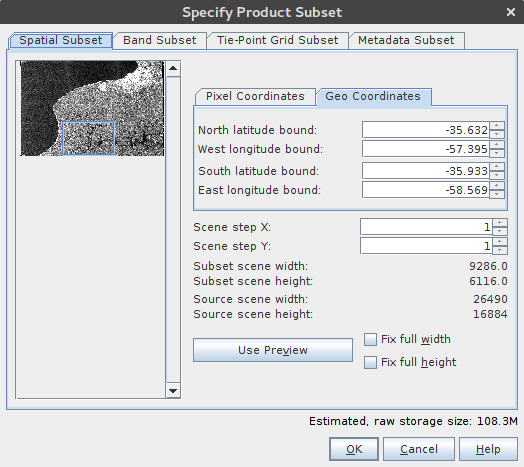
\includegraphics{fig:coordenadas.png}
        \caption{}
        \label{}
    \end{figure}
\end{que}

\begin{que}
    Procese la imagen como se vio en la clase 3. Calibrela para obtener el coeficiente de backscatter, aplique los filtros correspondientes y proyectela en terreno utilizando un DEM.
\end{que}

\begin{que}
    Identifique en la imagen cuerpos de agua, vegetados y ciudades. Mida su coeficiente de retrodispersión.
\end{que}

\begin{que}
    Utilizando la herramienta \emph{Analysis, Histogram} cálcule el histograma de la imagen e identifique un valor por debajo del cual el coeficiente de retrodispersión corresponde a agua.
\end{que}

\begin{que}
    Obtenga un mapa de zonas con agua. Para eso utilice la herramienta \emph{Band maths...} que se obtiene haciendo click derecho sobre la imagen y la formula
    \begin{verbatim}
        255*(Amplitude < T)
    \end{verbatim}
    donde T es el valor que obtuvo en el punto anterior.
\end{que}

\begin{que}
    Repita el proceso para la imagen \path{S1B_IW_GRDH_1SDV_20170318T094500_20170318T094525_004761_008514_AA78} previa a la inundacion
\end{que}
